\en{
Let $ABC$ be an acute triangle, and $I$ its incenter. Let $A_1$ be the intersection of $AI$ and $BC$, and $C_1$ the intersection of $CI$ and $AB$. Furthermore, let $M$ and $N$ be the midpoints of $AI$ and $CI$, respectively. Inside the triangles $AC_1I$ and $A_1CI$ we choose points $K$ and $L$ such that $\angle AKI = \angle CLI = \angle AIC$, $\angle AKM = \angle ICA$ and $\angle CLN = \angle IAC$. Prove that the radii of the circumcircles of the triangles $KIL$ and $ABC$ are equal.

\bigskip

\textbf{Solution (Marco):} Let $M_A$ and $M_C$ be the second intersections of the circle $(ABC)$ with $AI$ and $CI$, respectively. By the incenter/excenter lemma, $M_AI=M_AB$ and $M_CI=M_CB$, so $M_AM_C$ is the perpendicular bisector of $BI$. Hence, the reflection of the circle $(ABC)$ over $M_AM_C$ is the circle $(M_AIM_C)$, and they have the same radius. This proves that if $K$ and $L$ are on the circle $(M_AIM_C)$, we are done.

Moreover, by the incenter/excenter lemma,
\[
\angle M_CAI=\angle M_CIA=180^\circ-\angle CIA=180^\circ-\angle IKA
\]
implies that both $M_CA$ and $M_CI$ are tangent to the circle $(AKI)$. By the symmedian lemma, $M_CK$ is the $K$-symmedian of triangle $AKI$, so that if $V$ is the intersection of $M_CK$ and $AI$, then $\angle IKV=\angle MKA$. Thus,
\begin{align*}
  \angle M_CKI+\angle IM_AM_C&=180^\circ-\angle IKV+\angle AM_AM_C\\
  &=180^\circ-\angle MKA+\angle ACM_C\\
  &=180^\circ -\angle ACI+\angle ACM_C\\
  &=180^\circ,  
\end{align*}
and $K$ is on the circle $(M_AIM_C)$, as desired. Similarly, introducing $W$, the intersection of $M_AL$ and $CI$, we see that $L$ is also on the circle $(M_AIM_C)$, proving that $(KIL)=(M_AIM_C)$ and finishing the problem.

\begin{center}
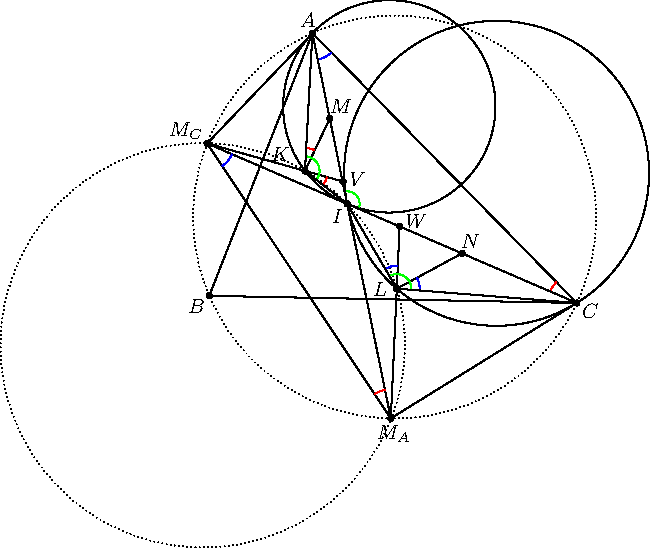
\includegraphics[scale=1.1]{2021/Selektion/muesterlosung/solutions/s12_fig.pdf}
\end{center}

\textbf{Marking Scheme (additive):}

\begin{enumerate}
    \item 1P: Introducing $M_A$ and $M_C$ in a sensible way, but only intersecting the circles $(ABC)$ and $(KIL)$ gives 0P.
    \item 1P: Claim that $(KIL)=(M_CIM_A)$, or prove that $(M_CIM_A)$ has the same radius as $(ABC)$.
    \item 2P: Prove that both $M_CA$ and $M_CI$ are tangent to $(AKI)$, or, similarly, that both $M_AC$ and $M_AI$ are tangent to $(CLI)$.
    \item 1P: Prove that $M_CK$ is the $K$-symmedian of $AKI$, or, similarly, that $M_AL$ is the $L$-symmedian of $CLI$.
    \item 2P: Conclude.
\end{enumerate}
}